\documentclass[10pt]{beamer}
% \setbeamersize{text margin left=10mm,text margin right=10mm}

% \usepackage[OT1]{fontenc}

\beamertemplatenavigationsymbolsempty

%\usefonttheme{professionalfonts}
% \usepackage{lxfonts}
% \usepackage{mathtools}
% \usepackage{lato}
% \usepackage{unicode-math}
% \setmainfont{Lato}
% \setmathfont{LatoMath.otf}

\usepackage{tikz, tikz-3dplot, tikz-cd, adjustbox, subcaption, changepage, mathtools, boldline, makecell, booktabs, graphicx}
\usetikzlibrary{knots, hobby, braids, decorations.markings, arrows.meta}
\usepackage{amsthm}
\usepackage{physics2}\usephysicsmodule{ab,ab.braket}

\usepackage{amsfonts, esint, slantsc, bboldx}
\usepackage{sansmathfonts}

\usetikzlibrary{cd, backgrounds}
\newcommand*\tmnl[2][c]{\begin{tabular}{@{}#1@{}}#2\end{tabular}}

\theoremstyle{definition}
\newtheorem{thm}{Theorem}

\newcommand{\I}{\mathbfbb{I}}
% \AtBeginDocument{\newcommand*\pii{\mathrm{π}}}
\newcommand{\R}{\mathbfbb{R}}
\newcommand{\C}{\mathbfbb{C}}
\newcommand{\Z}{\mathbfbb{Z}}

% \renewcommand*{\hbar}{\mathrm{^^^^0127}}
\renewcommand{\i}{\mathrm{i}}
% \newcommand{\I}{\mathbfbb{I}}
\newcommand{\ssep}{\mid}
\newcommand{\B}{\mathrm{B}}
\newcommand{\U}{\mathrm{U}}
\newcommand{\GB}{\text{GB}}
\newcommand{\TL}{\text{TL}}
% \newcommand{\sigmaa}{\mathrm{\sigma}}
% \newcommand{\tauu}{\mathrm{\tau}}
% \newcommand{\U}{\mathrm{U}}
% \DeclarePairedDelimiterX\presentation[1]\langle\rangle{\def\given{\;\delimsize\vert\;}#1}
\DeclarePairedDelimiter\abs{\lvert}{\rvert}
\DeclarePairedDelimiterX\set[1]\lbrace\rbrace{\setaux#1}
\def\setaux#1|{#1\;\delimsize\vert\;}
\DeclarePairedDelimiter{\norm}{\lVert}{\rVert}
\DeclarePairedDelimiter{\bracket}{\left\langle}{\right\rangle}
\makeatletter
\def\bign#1{\mathclose{\hbox{$\left#1\vbox to8.5\p@{}\right.\n@space$}}\mathopen{}}
\makeatother

%\newcommand{\e}{\mathrm{e}}
%\newcommand{\M}{\mathrm{M}}
% \newcommand{\upphi}{\mathrm{\phi}}
% \newcommand{\upPhii}{\mathrm{\Phi}}
% \newcommand{\updelta}{\mathrm{\delta}}
% \newcommand{\uprho}{\mathrm{\rho}}
\DeclareMathOperator{\tr}{tr}
% \DeclareMathOperator{\uprhoo}{\uprho}
% \DeclareMathOperator{\proj}{\pi}

\newcommand\restr[2]{{% we make the whole thing an ordinary symbol
		\left.\kern-\nulldelimiterspace % automatically resize the bar with \right
		#1 % the function
		\littletaller % pretend it's a little taller at normal size
		\right|_{#2} % this is the delimiter
	}}

\title{Braids and the bracket polynomial}
\subtitle{Thesis presentation}
\author{Apoorv Potnis}
\institute{IISERB}
\date{April 17, 2023}

% \AtBeginSection[]
% {
% 	\begin{frame}
% 		\frametitle{Table of Contents}
% 		\tableofcontents[currentsection, currentsubsection]
% 	\end{frame}
% 	\frame{\sectionpage}
% }
% \AtBeginSubsection{\frame{\subsectionpage}}

\newsavebox{\foobox}
\newcommand{\slantbox}[2][0]{\mbox{%
		\sbox{\foobox}{#2}%
		\hskip\wd\foobox
		\pdfsave
		\pdfsetmatrix{1 0 #1 1}%
		\llap{\usebox{\foobox}}%
		\pdfrestore
	}}
\newcommand\unslant[2][-.25]{\slantbox[#1]{$#2$}}
\newcommand{\sigmaa}{\unslant\sigma\!}
\newcommand{\updelta}{\unslant\delta\!}
\newcommand{\uprho}{\unslant\rho\!}
\DeclareMathOperator{\uprhoo}{\uprho}

\definecolor{beamer@blended}{rgb}{0.2,0.2,0.7}

\newcommand{\KP}[1]{%
	\begin{tikzpicture}[baseline=-\dimexpr\fontdimen22\textfont2\relax]
		#1
	\end{tikzpicture}%
}
\newcommand{\BPB}{
	\KP{
		\draw[line width=0.7pt] (-0.3,0.3) -- (0.3,-0.3);
		\draw[line width=0.7pt] (-0.3,-0.3) -- (-0.05,-0.05);
		\draw[line width=0.7pt] (0.05,0.05) -- (0.3,0.3);
		\draw[line width=0.7pt] (-0.45,-0.32) -- (-0.45,0.32);
		\node at (-0.7,0) {\(\cdots\)};
		\draw[line width=0.7pt] (-0.95,-0.32) -- (-0.95,0.32);
		\draw[line width=0.7pt] (0.45,-0.32) -- (0.45,0.32);
		\node at (0.7,0) {\(\cdots\)};
		\draw[line width=0.7pt] (0.95,-0.32) -- (0.95,0.32);
	}
}
\newcommand{\BPD}{
	\KP{
		\draw[line width=0.7pt] (-0.3,0.3) .. controls (0,-0.05) .. (0.3,0.3);
		\draw[line width=0.7pt] (-0.3,-0.3) .. controls (0,0.05) .. (0.3,-0.3);
		\draw[line width=0.7pt] (-0.45,-0.32) -- (-0.45,0.32);
		\node at (-0.7,0) {\(\cdots\)};
		\draw[line width=0.7pt] (-0.95,-0.32) -- (-0.95,0.32);
		\draw[line width=0.7pt] (0.45,-0.32) -- (0.45,0.32);
		\node at (0.7,0) {\(\cdots\)};
		\draw[line width=0.7pt] (0.95,-0.32) -- (0.95,0.32);
	}
}
\newcommand{\BPE}{
	\KP{
		\draw[line width=0.7pt] (-0.3,-0.3) .. controls (0.05,0) .. (-0.3,0.3);
		\draw[line width=0.7pt] (0.3,-0.3) .. controls (-0.05,0) .. (0.3,0.3);
		\draw[line width=0.7pt] (-0.45,-0.32) -- (-0.45,0.32);
		\node at (-0.7,0) {\(\cdots\)};
		\draw[line width=0.7pt] (-0.95,-0.32) -- (-0.95,0.32);
		\draw[line width=0.7pt] (0.45,-0.32) -- (0.45,0.32);
		\node at (0.7,0) {\(\cdots\)};
		\draw[line width=0.7pt] (0.95,-0.32) -- (0.95,0.32);
	}
}



\begin{document}

	\setbeamertemplate{caption}{\raggedright\insertcaption\par}

	\maketitle

% 	\begin{frame}
% 	    \tableofcontents
% 	\end{frame}

	\section{Outline}

	\begin{frame}[fragile]\vspace{1em}
		\begin{adjustwidth}{-0.5em}{-1.4em}
		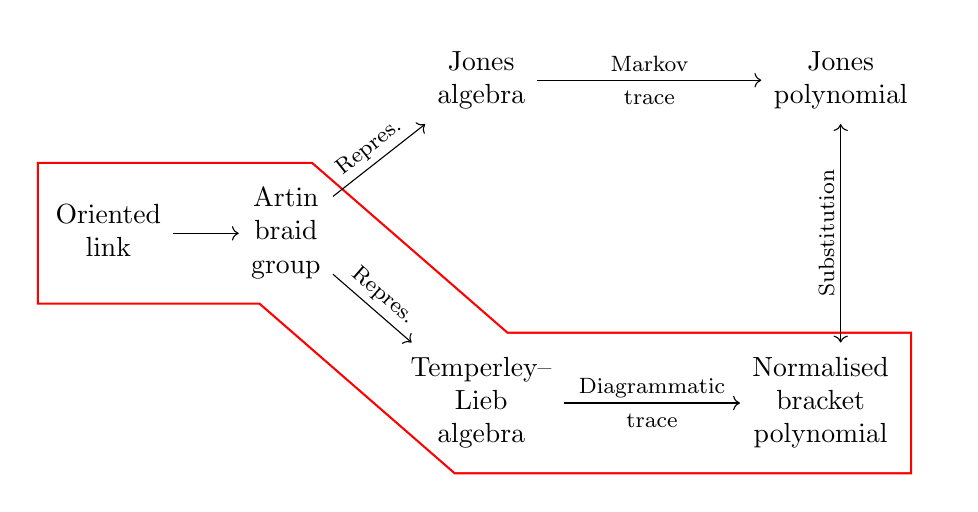
\begin{tikzpicture}[baseline= (a).base]
			\node[scale=1] (a) at (0,0){
				\begin{tikzcd}[
					math mode=false, labels={align=center},
					execute at end picture={
						\scoped[on background layer]
						\draw[red, thick, name prefix=\tikzcdmatrixname-,
						double distance=5em, line cap=rect]
						plot coordinates {(2-1)(2-2)(3-3)(3-4)};}]
					&
					&      \tmnl{Jones \\ algebra}        \arrow[r, "{\footnotesize Markov\\ \footnotesize trace}" auto=false]
					&[4em] \tmnl{Jones \\ polynomial} \\
					\tmnl{Oriented \\ link}        \arrow[r]
					&      \tmnl{Artin \\ braid \\ group} \arrow[rd, sloped, "{\footnotesize Repres.}"]
					\arrow[ru, sloped, "{\footnotesize Repres.}"] \\
					&
					& \tmnl{Temperley-- \\ Lieb \\ algebra}
					\arrow[r, "{\footnotesize Diagrammatic\\ \footnotesize trace}"' auto=false]
					& \tmnl{Normalised\phantom{asd} \\ bracket\phantom{asd} \\ polynomial\phantom{asd}}
					\arrow[uu, leftrightarrow, sloped, "{\footnotesize Substitution}"]
				\end{tikzcd}
			};
		\end{tikzpicture}
		\end{adjustwidth}

	\end{frame}

	\section{Braids}

	\subsection{Geometric definition}

	\begin{frame}
		\frametitle{Three dimensional representation}
		\begin{figure}
		    \centering
			\begin{tikzpicture}
				[scale=1.2,
				cube/.style={thick,black},
				grid/.style={very thin,gray},
				axis/.style={->,beamer@blendedblue,thick}]

				\draw[axis] (0,0,0) -- (6,0,0) node[anchor=west]{$x$};
				\draw[axis] (0,0,0) -- (0,3,0) node[anchor=south]{$y$};
				\draw[axis] (0,0,0) -- (0,0,3) node[anchor=north east]{$z$};

				%draw the top and bottom of the cube
				\draw[cube] (0,0,-1) -- (0,2,-1) -- (5,2,-1) -- (5,0,-1) -- cycle;


				%draw the edges of the cube
				\draw[cube] (0,0,-1) -- (0,0,1);
				\draw[cube] (0,2,-1) -- (0,2,1);
				\draw[cube] (5,0,-1) -- (5,0,1);
				\draw[cube] (5,2,-1) -- (5,2,1);

				\begin{knot}[clip width=8]
					\strand[thick, red] (1,0,0) to [in angle=-90, curve through = {(1.3,0.7,0.5)}] (4,2,0) node[black, below]{\(p_1\)};
					\strand[thick, red] (2,0,0) to [in angle=-90, curve through = {(1.3,1.5,0.5)}] (1,2,0) node[black, below]{\(p_2\)};
					\strand[thick, red] (3,0,0) to [in angle=-90, curve through = {(3,0.5,0.7)}] (2,2,0) node[black, below]{\(p_3\)};
					\strand[thick, red] (4,0,0) to [in angle=-90, curve through = {(3.2,1.3,-0.5)}] (3,2,0) node[black, below]{\(p_4\)};
					\flipcrossings{2}
				\end{knot}

				\node[below, label={\(q_1\)}] at (1,2,0) {};
				\node[below, label={\(q_2\)}] at (2,2,0) {};
				\node[below, label={\(q_3\)}] at (3,2,0) {};
				\node[below, label={\(q_4\)}] at (4,2,0) {};
% 				\node[left, label={O}] at (-0.05,-0.1,0) {};

				\draw[cube] (0,0,+1) -- (0,2,+1) -- (5,2,+1) -- (5,0,+1) -- cycle;

			\end{tikzpicture}
			\caption**{Three dimensional geometric representation of a braid}
		\end{figure}
	\end{frame}

	\begin{frame}
		\begin{figure}
			\frametitle{Two dimensional representation}
			\centering
			\begin{tikzpicture}
				[scale=1.5,
				cube/.style={thick,black},
				grid/.style={very thin,gray},
				axis/.style={->,beamer@blendedblue,thick}]

				\draw[axis] (0,0,0) -- (5,0) node[anchor=west]{\(x\)};
				\draw[axis] (0,0,0) -- (0,2.8) node[anchor=south]{\(y\)};

				\begin{knot}[clip width=8]
					\strand[thick, red] (1,0) to [in angle=-90, out angle=90, curve through = {(1.3,0.4)}] (4,2) node[black, below]{\(p_1\)};
					\strand[thick, red] (2,0) to [in angle=-90, out angle=90, curve through = {(1.3,1.2)}] (1,2) node[black, below]{\(p_2\)};
					\strand[thick, red] (3,0) to [in angle=-90, out angle=90, curve through = {(2.8,0.5)}] (2,2) node[black, below]{\(p_3\)};
					\strand[thick, red] (4,0) to [in angle=-90, out angle=90, curve through = {(3.2,1.6)}] (3,2) node[black, below]{\(p_4\)};
					\flipcrossings{2}
				\end{knot}

				\node[below, label={\(q_1\)}] at (1,2) {};
				\node[below, label={\(q_2\)}] at (2,2) {};
				\node[below, label={\(q_3\)}] at (3,2) {};
				\node[below, label={\(q_4\)}] at (4,2) {};
			\end{tikzpicture}
			\caption**{A projection of the braid}
			\label{fig:2drepbraids}
		\end{figure}
	\end{frame}

	\begin{frame}
		\frametitle{Multiplication of braids}
		\begin{figure}
			\centering
			\subcaptionbox*{\(b_1\)}{
				
\begin{tikzpicture}[scale=1]
					\begin{knot}[clip width=8]
						\strand[thick, red] (1,0) to [in angle=-90, out angle=90, curve through = {(1.5,0.5)}] (1,2);
						\strand[thick, red] (2,0) to [in angle=-90, out angle=90, curve through = {(1.9,0.5)}] (3,2);
						\strand[thick, red] (3,0) to [in angle=-90, out angle=90, curve through = {(2,1.3)}] (2,2);
					\end{knot}
				\end{tikzpicture}\label{fig:braidmultiplication1}}\qquad\quad
			\subcaptionbox*{\(b_2\)}{
				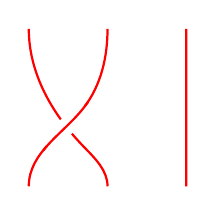
\begin{tikzpicture}[scale=1]
					\begin{knot}[clip width=8]
						\strand[thick, red] (1,0) to [in angle=-90, out angle=90, curve through = {(1.7,1)}] (2,2);
						\strand[thick, red] (2,0) to [in angle=-90, out angle=90, curve through = {(1.7,0.5)}] (1,2);
						\strand[thick, red] (3,0) to [in angle=-90, out angle=90, curve through = {(3,0.5)}] (3,2);
					\end{knot}
				\end{tikzpicture}\label{fig:braidmultiplication2}}\quad\quad\quad
			\subcaptionbox*{\(b_1 b_2\)}{
				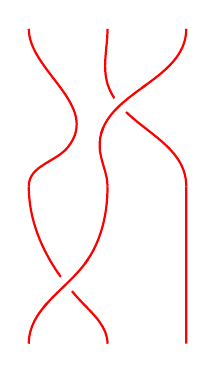
\begin{tikzpicture}[scale=1]
					\begin{knot}[clip width=8]
						\strand[thick, red] (1,0) to [in angle=-90, out angle=90, curve through = {(1.7,1)}] (2,2);
						\strand[thick, red] (2,0) to [in angle=-90, out angle=90, curve through = {(1.7,0.5)}] (1,2);
						\strand[thick, red] (3,0) to [in angle=-90, out angle=90, curve through = {(3,0.5)}] (3,2);
						\strand[thick, red] (1,2) to [in angle=-90, out angle=90, curve through = {(1.5,2.5)}] (1,4);
						\strand[thick, red] (2,2) to [in angle=-90, out angle=90, curve through = {(1.9,2.5)}] (3,4);
						\strand[thick, red] (3,2) to [in angle=-90, out angle=90, curve through = {(2,3.3)}] (2,4);
					\end{knot}
				\end{tikzpicture}\label{fig:braidmultiplication3}}
			\caption*{Multiplication of two braids}\label{fig:braidmultiplication}
		\end{figure}
	\end{frame}

	\begin{frame}
		\frametitle{The identity braid \(\I_n\)}
		\begin{figure}\centering
			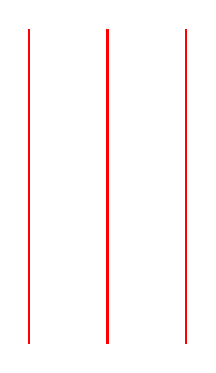
\begin{tikzpicture}[scale=1]
				\begin{knot}[yscale=2, clip width=8]
					\strand[thick, red] (1,0) to (1,2);
					\strand[thick, red] (2,0) to (2,2);
					\strand[thick, red] (3,0) to (3,2);
% 					\flipcrossings{2}
				\end{knot}
			\end{tikzpicture}
			\caption*{The identity \(\I_3\)}
			\label{fig:braididentity}
		\end{figure}
	\end{frame}

	\begin{frame}
		\frametitle{Inverse of braids}
		\begin{figure}
			\centering
			\subcaptionbox*{\(b\)}{
				
\begin{tikzpicture}[scale=1]
					\begin{knot}[clip width=8]
						\strand[thick, red] (1,0) to [in angle=-90, out angle=90, curve through = {(1.5,0.5)}] (1,2);
						\strand[thick, red] (2,0) to [in angle=-90, out angle=90, curve through = {(1.9,0.5)}] (3,2);
						\strand[thick, red] (3,0) to [in angle=-90, out angle=90, curve through = {(2,1.3)}] (2,2);
						\flipcrossings{2}
					\end{knot}
				\end{tikzpicture}\label{fig:braidinverse1}}\qquad\quad
			\subcaptionbox*{\(b^{-1}\)}{
				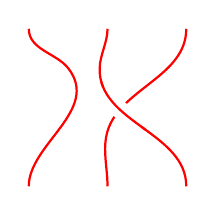
\begin{tikzpicture}[scale=1]
					\begin{knot}[clip width=8, yscale=-1]
						\strand[thick, red] (1,0) to [in angle=-90, out angle=90, curve through = {(1.5,0.5)}] (1,2);
						\strand[thick, red] (2,0) to [in angle=-90, out angle=90, curve through = {(1.9,0.5)}] (3,2);
						\strand[thick, red] (3,0) to [in angle=-90, out angle=90, curve through = {(2,1.3)}] (2,2);
						\flipcrossings{2}
					\end{knot}
				\end{tikzpicture}\label{fig:braidinverse2}}\quad\quad\quad
			\subcaptionbox*{\(b b^{-1} = \I_3\)}{
				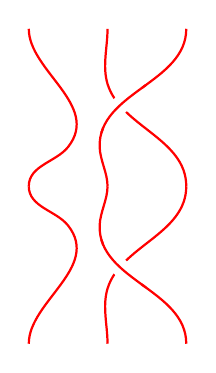
\begin{tikzpicture}[scale=1]
					\begin{knot}[clip width=8]
						\strand[thick, red] (1,0) to [in angle=-90, out angle=90, curve through = {(1.5,0.5)}] (1,2);
						\strand[thick, red] (2,0) to [in angle=-90, out angle=90, curve through = {(1.9,0.5)}] (3,2);
						\strand[thick, red] (3,0) to [in angle=-90, out angle=90, curve through = {(2,1.3)}] (2,2);
						\flipcrossings{2}
						\begin{scope}
							\begin{knot}[clip width=8, yscale=-1]
								\strand[thick, red] (1,0) to [in angle=-90, out angle=90, curve through = {(1.5,0.5)}] (1,2);
								\strand[thick, red] (2,0) to [in angle=-90, out angle=90, curve through = {(1.9,0.5)}] (3,2);
								\strand[thick, red] (3,0) to [in angle=-90, out angle=90, curve through = {(2,1.3)}] (2,2);
								\flipcrossings{2}
							\end{knot}
						\end{scope}
					\end{knot}
				\end{tikzpicture}\label{fig:braidinverse3}}
% 			\quad\quad
% 			\subcaptionbox*{\(\I_3\)}{
% 				\begin{tikzpicture}[scale=0.8]
% 					\begin{knot}[clip width=8, yscale=2]
% 						\strand[thick, red] (1,0) to (1,2);
% 						\strand[thick, red] (2,0) to (2,2);
% 						\strand[thick, red] (3,0) to (3,2);
% 						% \flipcrossings{2}
% 					\end{knot}
%
% 					%\node[below, label={\(q_1''\)}] at (1,4) {};
% 					%\node[below, label={\(q_2''\)}] at (2,4) {};
% 					%\node[below, label={\(q_3''\)}] at (3,4) {};
%
% 					%\node at (2, -1.2) {\(b_1 b_2\)};
% 				\end{tikzpicture}\label{fig:braidinverse4}}
			\caption*{Inverse of a braid}\label{fig:braidinverse}
		\end{figure}
	\end{frame}

	\begin{frame}
	    Thus, braids form a group, known as the Artin braid group \(\B_n\).
	\end{frame}

	\subsection{Generators and relations}

	\begin{frame}\vspace{1em}
		\frametitle{Generators of the braid group}
		\begin{figure}
			\centering
			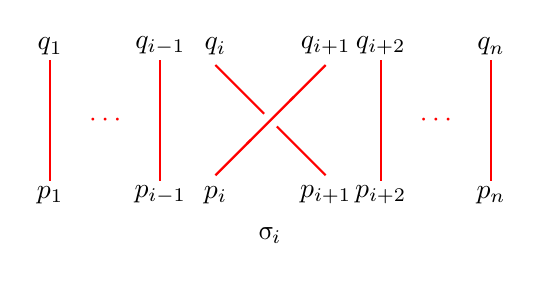
\begin{tikzpicture}[scale=0.7]
				\begin{knot}[clip width=8]
					\strand[thick, red] (-3,-0.1) to (-3,2.1);
					\strand[thick, red] (-1,-0.1) to (-1,2.1);
					\strand[thick, red] (0,0) to (2,2);
					\strand[thick, red] (2,0) to (0,2);
					\strand[thick, red] (3,-0.1) to (3,2.1);
					\strand[thick, red] (5,-0.1) to (5,2.1);
				\end{knot}
				\node[ultra thick, red] at (-2,1) {\(\cdots\)};
				\node[ultra thick, red] at (4,1) {\(\cdots\)};

				\node[below, label={\(p_1\)}] at (-3,-0.7) {};
				\node[below, label={\(p_{i-1}\)}] at (-1,-0.7) {};
				\node[below, label={\(q_1\)}] at (-3,2) {};
				\node[below, label={\(q_{i-1}\)}] at (-1,2) {};
				\node[below, label={\(q_i\)}] at (0,2) {};
				\node[below, label={\(q_{i+1}\)}] at (2,2) {};
				\node[below, label={\(p_i\)}] at (0,-0.7) {};
				\node[below, label={\(p_{i+1}\)}] at (2,-0.7) {};
				\node[below, label={\(p_{i+2}\)}] at (3,-0.7) {};
				\node[below, label={\(p_{n}\)}] at (5,-0.7) {};
				\node[below, label={\(q_{i+2}\)}] at (3,2) {};
				\node[below, label={\(q_{n}\)}] at (5,2) {};

				\node at (1, -1.1) {\(\sigmaa_i\)};

				\end{tikzpicture}

				\vspace{12pt}

				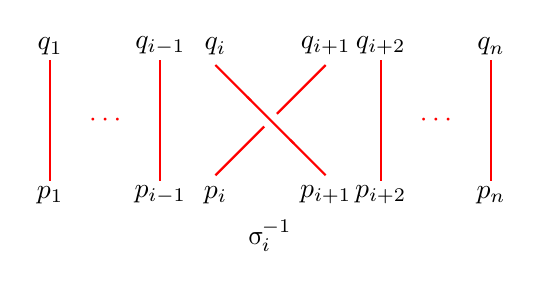
\begin{tikzpicture}[scale=0.7]
					\begin{knot}[clip width=8]
						\strand[thick, red] (-3,-0.1) to (-3,2.1);
						\strand[thick, red] (-1,-0.1) to (-1,2.1);
						\strand[thick, red] (0,0) to (2,2);
						\strand[thick, red] (2,0) to (0,2);
						\strand[thick, red] (3,-0.1) to (3,2.1);
						\strand[thick, red] (5,-0.1) to (5,2.1);
						\flipcrossings{1}
					\end{knot}
					\node[ultra thick, red] at (-2,1) {\(\cdots\)};
					\node[ultra thick, red] at (4,1) {\(\cdots\)};

					\node[below, label={\(p_1\)}] at (-3,-0.7) {};
					\node[below, label={\(p_{i-1}\)}] at (-1,-0.7) {};
					\node[below, label={\(q_1\)}] at (-3,2) {};
					\node[below, label={\(q_{i-1}\)}] at (-1,2) {};
					\node[below, label={\(q_i\)}] at (0,2) {};
					\node[below, label={\(q_{i+1}\)}] at (2,2) {};
					\node[below, label={\(p_i\)}] at (0,-0.7) {};
					\node[below, label={\(p_{i+1}\)}] at (2,-0.7) {};
					\node[below, label={\(p_{i+2}\)}] at (3,-0.7) {};
					\node[below, label={\(p_{n}\)}] at (5,-0.7) {};
					\node[below, label={\(q_{i+2}\)}] at (3,2) {};
					\node[below, label={\(q_{n}\)}] at (5,2) {};

					\node at (1, -1.1) {\(\sigmaa_i^{-1}\)};
				\end{tikzpicture}

			\caption*{Generators \(\sigmaa_i\) and \(\sigmaa_i^{-1}\)}
			\label{fig:geometricbraidgenerators}
		\end{figure}
	\end{frame}

	\begin{frame}
		\frametitle{Type II move: \(\sigmaa_i\hspace{1pt} \sigmaa_i^{-1} = \I_n\)}
		\begin{figure}
			\centering
			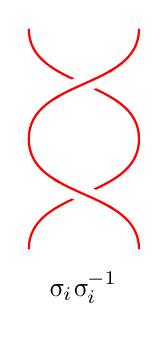
\begin{tikzpicture}
				[scale=0.7]

				\begin{knot}[clip width=8]
					\strand[thick, red] (0,0) to [in angle=-90, out angle=90, curve through = {(2,2)}] (0,4);
					\strand[thick, red] (2,0) to [in angle=-90, out angle=90, curve through = {(0,2)}] (2,4);
					\flipcrossings{1,2}
				\end{knot}

				\node at (1, -0.7) {\(\sigmaa_i\hspace{1pt} \sigmaa_i^{-1}\)};
			\end{tikzpicture}
			\quad\quad\quad\quad
			\begin{tikzpicture}
				[scale=0.7]

				\begin{knot}[clip width=8]
					\strand[thick, red] (0,0) to (0,4);
					\strand[thick, red] (2,0) to (2,4);
					\flipcrossings{1,2}
				\end{knot}

				\node at (1, -0.7) {\(\I_n\)};
			\end{tikzpicture}

			\caption*of{figure}{A type II move illustrating \(\sigmaa_i\hspace{1pt} \sigmaa_i^{-1} = \I_n\)}
			\label{fig:type2}
		\end{figure}
	\end{frame}


	\begin{frame}
		\frametitle{Type III move: \(\sigmaa_i\hspace{1pt} \sigmaa_{i+1} \sigmaa_i = \sigmaa_{i+1} \sigmaa_i\hspace{1pt} \sigmaa_{i+1}\)}
		\begin{figure}\centering
			\begin{tikzpicture}
				[scale=0.6]

				\begin{knot}[clip width=6]
					\strand[ultra thick, beamer@blendedblue] (0,0) to [in angle=-90, out angle=90, curve through = {(2,2) (4,4)}] (4,6);
					\strand[thick, red] (2,0) to [in angle=-90, out angle=90, curve through = {(0,2) (0,4)}] (2,6);
					\strand[thick, red] (4,0) to [in angle=-90, out angle=90, curve through = {(4,2) (2,4)}] (0,6);
				\end{knot}

				\node at (2, -0.7) {\(\sigmaa_i\hspace{1pt} \sigmaa_{i+1} \sigmaa_i\)};
			\end{tikzpicture}
			\quad\quad\quad\quad
			\begin{tikzpicture}
				[scale=0.6]

				\begin{knot}[clip width=6]
					\strand[ultra thick, beamer@blendedblue] (0,0) to [in angle=-90, out angle=90, curve through = {(0,2) (2,4)}] (4,6);
					\strand[thick, red] (2,0) to [in angle=-90, out angle=90, curve through = {(4,2) (2,4)}] (2,6);
					\strand[thick, red] (4,0) to [in angle=-90, out angle=90, curve through = {(2,2) (0,4)}] (0,6);
					%\flipcrossings{1,2}
				\end{knot}

				\node at (2, -0.7) {\(\sigmaa_{i+1} \sigmaa_i\hspace{1pt} \sigmaa_{i+1}\)};
			\end{tikzpicture}

			\caption*of{figure}{A type III move illustrating \(\sigmaa_i\hspace{1pt} \sigmaa_{i+1} \sigmaa_i = \sigmaa_{i+1} \sigmaa_i\hspace{1pt} \sigmaa_{i+1}\)}
			\label{fig:type3}
		\end{figure}
	\end{frame}

	\begin{frame}
		\frametitle{Sliding of crossings: \(\sigmaa_i\hspace{1pt} \sigmaa_j = \sigmaa_j\hspace{1pt} \sigmaa_i\)}
		\begin{figure}\centering
			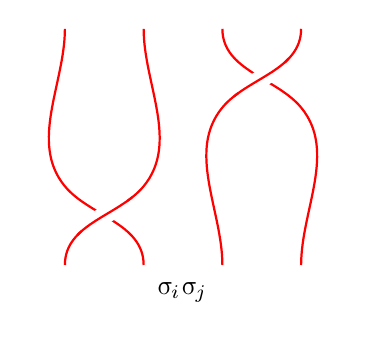
\begin{tikzpicture}
				[scale=0.5]

				\begin{knot}[clip width=8]
					\strand[thick, red] (0,0) to [in angle=-90, out angle=90, curve through = {(2,2)}] (2,6);
					\strand[thick, red] (2,0) to [in angle=-90, out angle=90, curve through = {(0,2)}] (0,6);
					\strand[thick, red] (4,0) to [in angle=-90, out angle=90, curve through = {(4,4)}] (6,6);
					\strand[thick, red] (6,0) to [in angle=-90, out angle=90, curve through = {(6,4)}] (4,6);
				\end{knot}

				\node at (3, -0.7) {\(\sigmaa_i\hspace{1pt} \sigmaa_j\)};
			\end{tikzpicture}
			\quad\quad\quad\quad
			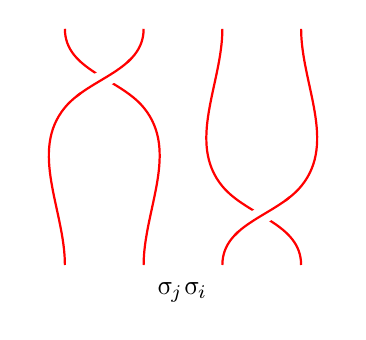
\begin{tikzpicture}
				[scale=0.5]

				\begin{knot}[clip width=8]
					\strand[thick, red] (0,0) to [in angle=-90, out angle=90, curve through = {(0,4)}] (2,6);
					\strand[thick, red] (2,0) to [in angle=-90, out angle=90, curve through = {(2,4)}] (0,6);
					\strand[thick, red] (4,0) to [in angle=-90, out angle=90, curve through = {(6,2)}] (6,6);
					\strand[thick, red] (6,0) to [in angle=-90, out angle=90, curve through = {(4,2)}] (4,6);
					%\flipcrossings{1,2}
				\end{knot}

				\node at (3, -0.7) {\(\sigmaa_j\hspace{1pt} \sigmaa_i\)};
			\end{tikzpicture}

			\caption*of{figure}{Sliding of crossings illustrating \(\sigmaa_i\hspace{1pt} \sigmaa_j = \sigmaa_j\hspace{1pt} \sigmaa_i\)}
			\label{fig:sliding}
		\end{figure}
	\end{frame}

	\subsection{Algebraic definition}

	\begin{frame}
		\frametitle{Presentation of the braid group}
		The Artin braid group \(\B_n\) admits the following presentation on the generators \(\sigmaa_i\), for \(1 \leq i \leq n-1 \).
		\[\B_n =\Biggl\langle
		\begin{array}{cV{1.5}rcll}
			& \sigmaa_i \hspace{1pt}\sigmaa_i^{-1} &=& \mathbfbb{I}_n &\\
			\sigmaa_1,\ldots, \sigmaa_{n-1} & \sigmaa_i\hspace{1pt} \sigmaa_{i+1} \sigmaa_i &=& \sigmaa_{i+1} \sigmaa_i\hspace{1pt} \sigmaa_{i+1} &\text{if } i+1 \leq n-1\\
			& \sigmaa_i\hspace{1pt} \sigmaa_j &=& \sigmaa_j \hspace{1pt}\sigmaa_i &\text{if } \abs{i-j} \geq 2
		\end{array}
		\Biggr\rangle\]
	\end{frame}

	\section{Closure}

	\subsection{Closure of a braid}

	\begin{frame}
		\frametitle{Closure of a braid \(\overline{b}\)}
		\begin{figure}\centering
			\raisebox{0cm}{\begin{tikzpicture}
					\begin{knot}[clip width=5]
						\strand[very thick, beamer@blendedblue] (1,1) to [out=90,in=-90, beamer@blendedblue] (0,2);
						\strand[very thick, beamer@blendedblue] (0,1) to [out=90,in=-90, beamer@blendedblue] (1,2);
						\flipcrossings{1,2}
% 						\strand[very thick, beamer@blendedblue] (0,0) to[in angle=-90, out angle=90, curve through = {(1,1)}] (2,2);
% 						\strand[very thick, beamer@blendedblue] (2,0) to[in angle=-90, out angle=90, curve through = {(1,1)}] (0,2);
% 						\strand[very thick, beamer@blendedblue] (4,0) to (4,2);
						%\strand[thick, red] (6,0) to [in angle=-90, out angle=90, curve through = {(6,4)}] (4,6);
					\end{knot}

					\node at (0.5, -0.5) {\(b\)};
				\end{tikzpicture}}\quad\quad\quad\quad
				\begin{tikzpicture}
					\begin{knot}[clip width = 5]
						\strand[thick, red] (0,2) to (0,3) to (2,3) to (2,0) to (0,0) to (0,1);
						\strand[thick, red] (1,2) to (1,2.5) to (1.5,2.5) to (1.5,0.5) to (1,0.5) to (1,1);
						\strand[very thick, beamer@blendedblue] (1,1) to [out=90,in=-90, beamer@blendedblue] (0,2);
						\strand[very thick, beamer@blendedblue] (0,1) to [out=90,in=-90, beamer@blendedblue] (1,2);
						\flipcrossings{1,2}
					\end{knot}
					\node at (1,-0.5) {\(\overline{b}\)};
				\end{tikzpicture}
			\caption*{Closure of a braid}
			\label{fig:closure}
		\end{figure}
	\end{frame}

	\begin{frame}
		\frametitle{Braids and links}
		Every closure of a braid is a link.
		\vspace{50pt}

		\begin{thm}[Alexander]
		    Every link is ambient isotopic to a closure of a braid.
		\end{thm}
	\end{frame}

	\subsection{Equivalence of closures of braids}

	\begin{frame}
		\frametitle{Conjugation}
		\begin{figure}
			\centering
				\begin{tikzpicture}[scale=1]
					\begin{knot}[clip width = 7]
						\strand[thick, red] (0,0) to [in=-90, out=90](1,1);
						\strand[thick, red] (0,2) to [out=90, in=-90](1,3) to (1,3.5) to (1.5,3.5) to (1.5,-0.5) to (1,-0.5) to (1,0);
						\strand[thick, red] (1,0) to [in=-90, out=90](0,1);
						\strand[thick, red] (1,2) to [out=90, in=-90](0,3) to (0,4) to (2,4) to (2,-1) to (0,-1) to (0,0);
						\strand[very thick, beamer@blendedblue] (1,1) to [out=90,in=-90, beamer@blendedblue] (0,2);
						\strand[very thick, beamer@blendedblue] (0,1) to [out=90,in=-90, beamer@blendedblue] (1,2);
						\flipcrossings{2}
					\end{knot}
					\node at (-0.5,0.5) {\(g^{-1}\)};
					\node at (-0.5,1.5) {\(b\)};
					\node at (-0.5,2.5) {\(g\)};
					\begin{scope}[xshift=4cm]
						\begin{knot}[clip width = 7]
							\strand[thick, red] (0,2) to (0,3.5) to (1.5,3.5) to (2.5,2.5) to (3,2.5) to (3,0.5) to (2.5,0.5) to (1.5,-0.5) to (0,-0.5) to (0,1);
							\strand[thick, red] (1,2) to (1,2.5) to (1.5,2.5) to (2.5,3.5) to (3.5,3.5) to (3.5,-0.5) to (2.5,-0.5) to (1.5,0.5) to (1,0.5) to (1,1);
							\strand[very thick, beamer@blendedblue] (1,1) to [out=90,in=-90, beamer@blendedblue] (0,2);
							\strand[very thick, beamer@blendedblue] (0,1) to [out=90,in=-90, beamer@blendedblue] (1,2);
							\flipcrossings{1,2}
						\end{knot}
						\node at (2,-1) {\(g^{-1}\)};
						\node at (-0.5,1.5) {\(b\)};
						\node at (2,4) {\(g\)};
					\end{scope}
				\end{tikzpicture}
% 				\par\medskip
% 			\subcaptionbox*{}{
% 				\begin{tikzpicture}[scale=0.6]
% 					\begin{knot}[clip width = 5]
% 						\strand[thick, red] (0,2) to (0,3.75) to (2.5,3.75) to (2.5,2.75) to (1.5,1.75) to (1.5,1.25) to (2.5,0.25) to (2.5,-0.75) to (0,-0.75) to (0,1);
% 						\strand[thick, red] (1,2) to (1,3.25) to (1.5,3.25) to (1.5,2.75) to (2.5,1.75) to (2.5,1.25) to (1.5,0.25) to (1.5,-0.25) to (1,-0.25) to (1,1);
% 						\strand[very thick, beamer@blendedblue] (1,1) to [out=90,in=-90, beamer@blendedblue] (0,2);
% 						\strand[very thick, beamer@blendedblue] (0,1) to [out=90,in=-90, beamer@blendedblue] (1,2);
% 						\flipcrossings{1,2}
% 					\end{knot}
% 					\node at (3,0.75) {\(g^{-1}\)};
% 					\node at (-0.5,1.5) {\(b\)};
% 					\node at (3,2.25) {\(g\)};
% 				\end{tikzpicture}}
% 			\qquad\subcaptionbox*{}{
% 				\begin{tikzpicture}[scale=0.6]
% 					\begin{knot}[clip width = 5]
% 						\strand[thick, red] (0,2) to (0,3) to (2,3) to (2,0) to (0,0) to (0,1);
% 						\strand[thick, red] (1,2) to (1,2.5) to (1.5,2.5) to (1.5,0.5) to (1,0.5) to (1,1);
% 						\strand[very thick, beamer@blendedblue] (1,1) to [out=90,in=-90, beamer@blendedblue] (0,2);
% 						\strand[very thick, beamer@blendedblue] (0,1) to [out=90,in=-90, beamer@blendedblue] (1,2);
% 						\flipcrossings{1,2}
% 					\end{knot}
% 					\node at (-0.5,1.5) {\(b\)};
% 				\end{tikzpicture}}
			\caption*{Conjugation process illustrating the link equivalence of \(\overline{g b g^{-1}}\) and \(\overline{b}\) (part 1)}
			\label{fig:conjugationone}
		\end{figure}
	\end{frame}

	\begin{frame}
		\frametitle{Conjugation (contd.)}
		\begin{figure}
		    \centering
			\begin{tikzpicture}[scale=1]
				\begin{knot}[clip width = 7]
					\strand[thick, red] (0,2) to (0,3.75) to (2.5,3.75) to (2.5,2.75) to (1.5,1.75) to (1.5,1.25) to (2.5,0.25) to (2.5,-0.75) to (0,-0.75) to (0,1);
					\strand[thick, red] (1,2) to (1,3.25) to (1.5,3.25) to (1.5,2.75) to (2.5,1.75) to (2.5,1.25) to (1.5,0.25) to (1.5,-0.25) to (1,-0.25) to (1,1);
					\strand[very thick, beamer@blendedblue] (1,1) to [out=90,in=-90, beamer@blendedblue] (0,2);
					\strand[very thick, beamer@blendedblue] (0,1) to [out=90,in=-90, beamer@blendedblue] (1,2);
					\flipcrossings{1,2}
				\end{knot}
				\node at (3,0.75) {\(g^{-1}\)};
				\node at (-0.5,1.5) {\(b\)};
				\node at (3,2.25) {\(g\)};
				\begin{scope}
					\begin{knot}[xshift = 5cm, clip width = 7]
						\node at (-0.5,1.5) {\(b\)};
						\strand[thick, red] (0,2) to (0,3) to (2,3) to (2,0) to (0,0) to (0,1);
						\strand[thick, red] (1,2) to (1,2.5) to (1.5,2.5) to (1.5,0.5) to (1,0.5) to (1,1);
						\strand[very thick, beamer@blendedblue] (1,1) to [out=90,in=-90, beamer@blendedblue] (0,2);
						\strand[very thick, beamer@blendedblue] (0,1) to [out=90,in=-90, beamer@blendedblue] (1,2);
						\flipcrossings{1,2}
					\end{knot}
				\end{scope}
			\end{tikzpicture}
			\caption*{Conjugation process illustrating the link equivalence of \(\overline{g b g^{-1}}\) and \(\overline{b}\) (part 2)}
			\label{fig:conjugationtwo}
		\end{figure}
	\end{frame}

	\begin{frame}
		\frametitle{Markov theorem}
		\begin{thm}[Markov]
			Two braids whose closures are ambient isotopic to each other are related by a finite sequence of the following operations.
			\begin{enumerate}
				\item Braid equivalences, i.e.\@ equivalences resulting due to the braid relations.
				\item Conjugation.
				\item Markov moves.
			\end{enumerate}
		\end{thm}
	\end{frame}

	\begin{frame}
		\frametitle{Markov move}
		\begin{figure}
			\centering
			\subcaptionbox*{}{
				\begin{tikzpicture}
					\begin{knot}[clip width = 5]
						\strand[thick, red] (0,2) to (0,3) to (2,3) to (2,0) to (0,0) to (0,1);
						\strand[thick, red] (1,2) to (1,2.5) to (1.5,2.5) to (1.5,0.5) to (1,0.5) to (1,1);
						\strand[very thick, beamer@blendedblue] (1,1) to [out=90,in=-90, beamer@blendedblue] (0,2);
						\strand[very thick, beamer@blendedblue] (0,1) to [out=90,in=-90, beamer@blendedblue] (1,2);
						\flipcrossings{2}
					\end{knot}
					\node at (-0.5,1.5) {\(b\)};
					\node at (1,-0.5) {\(\overline{b}\)};
				\end{tikzpicture}}
			\quad\quad\quad\subcaptionbox*{}{
				\begin{tikzpicture}
					\begin{knot}[clip width = 5]
						\strand[very thick, beamer@blendedblue] (0,0) to (0,1) to [out=90,in=-90, beamer@blendedblue] (1,2);
						\strand[thick, red] (1,2) to (1,3) to (3,3) to (3,-1) to (1,-1) to (1,0);
						\strand[very thick, beamer@blendedblue] (1,0) to [out=90,in=-90, beamer@blendedblue] (2,1) to (2,2);
						\strand[thick, red] (2,2) to (2,2.5) to (2.5,2.5) to (2.5,-0.5) to (2,-0.5) to (2,0);
						\strand[very thick, beamer@blendedblue] (2,0) to [out=90,in=-90, beamer@blendedblue]  (1,1) to [out=90,in=-90, beamer@blendedblue] (0,2);
						\strand[thick, red] (0,2) to (0,3.5) to (3.5,3.5) to (3.5,-1.5) to (0,-1.5) to (0,0);
						\flipcrossings{1}
					\end{knot}
					\node at (1.75,-2) {\(\overline{b\hspace{1pt}\sigmaa_2}\)};
				\end{tikzpicture}}
			\caption*{Markov move with \(b = \sigmaa_1^{-1}\).}
			\label{fig:markovmove}
		\end{figure}
	\end{frame}

	\section{Orientation}

	\begin{frame}
		\frametitle{Orientation}
		\begin{figure}
			\centering
			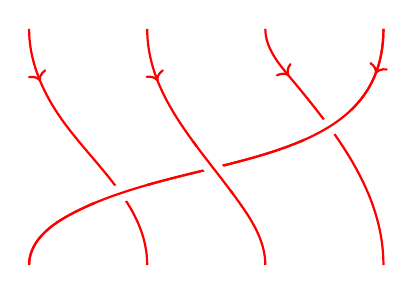
\begin{tikzpicture}
				[scale=1.5,
				cube/.style={thick,black},
				grid/.style={very thin,gray},
				axis/.style={->,beamer@blendedblue,thick}]

% 				\draw[axis] (0,0,0) -- (5,0) node[anchor=west]{\(x\)};
% 				\draw[axis] (0,0,0) -- (0,2.8) node[anchor=south]{\(y\)};

				\begin{knot}[clip width=8]
					\strand[thick, red, draw=red,
					only when rendering/.style={
						postaction=decorate,
					},
					decoration={
						markings,
						mark=at position .9 with {\arrowreversed{To}}
					}] (1,0) to [in angle=-90, out angle=90, curve through = {(1.3,0.4)}] (4,2);% node[black, below]{\(p_1\)};
					\strand[thick, red,
					only when rendering/.style={
						postaction=decorate,
					},
					decoration={
						markings,
						mark=at position .8 with {\arrowreversed{To}}
					}] (2,0) to [in angle=-90, out angle=90, curve through = {(1.3,1.2)}] (1,2);% node[black, below]{\(p_2\)};
					\strand[thick, red,
					only when rendering/.style={
						postaction=decorate,
					},
					decoration={
						markings,
						mark=at position .8 with {\arrowreversed{To}}
					}] (3,0) to [in angle=-90, out angle=90, curve through = {(2.8,0.5)}] (2,2);% node[black, below]{\(p_3\)};
					\strand[thick, red,
					only when rendering/.style={
						postaction=decorate,
					},
					decoration={
						markings,
						mark=at position .8 with {\arrowreversed{To}}
					}] (4,0) to [in angle=-90, out angle=90, curve through = {(3.2,1.6)}] (3,2);% node[black, below]{\(p_4\)};
					\flipcrossings{2}
				\end{knot}

% 				\node[below, label={\(q_1\)}] at (1,2) {};
% 				\node[below, label={\(q_2\)}] at (2,2) {};
% 				\node[below, label={\(q_3\)}] at (3,2) {};
% 				\node[below, label={\(q_4\)}] at (4,2) {};
			\end{tikzpicture}
			\caption*{A 	braid with downward orientation}
			\label{fig:2drepbraidsorientation}
		\end{figure}
	\end{frame}

	\begin{frame}
		%\frametitle{}
		For the consistency of the orientation, it must be either upwards or downwards for all strands.\vspace{1.5em}

		\begin{figure}
			\centering\captionsetup[subfigure]{justification=centering}
			\subcaptionbox*{\(\sigmaa_i\) gets assigned \(+1\)}{
			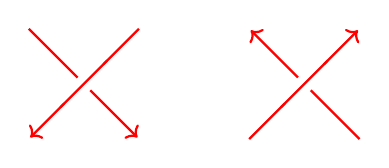
\begin{tikzpicture}[scale=0.7]
				\begin{knot}[clip width=8]
% 					\strand[thick, red] (-3,-0.1) to (-3,2.1);
% 					\strand[thick, red] (-1,-0.1) to (-1,2.1);
					\strand[thick, red, <-] (0,0) to (2,2);
					\strand[thick, red, <-] (2,0) to (0,2);
					\strand[thick, red, ->] (4,0) to (6,2);
					\strand[thick, red, ->] (6,0) to (4,2);
% 					\strand[thick, red] (3,-0.1) to (3,2.1);
% 					\strand[thick, red] (5,-0.1) to (5,2.1);
				\end{knot}
% 				\node[ultra thick, red] at (-2,1) {\(\cdots\)};
% 				\node[ultra thick, red] at (4,1) {\(\cdots\)};
%
% 				\node[below, label={\(p_1\)}] at (-3,-0.7) {};
% 				\node[below, label={\(p_{i-1}\)}] at (-1,-0.7) {};
% 				\node[below, label={\(q_1\)}] at (-3,2) {};
% 				\node[below, label={\(q_{i-1}\)}] at (-1,2) {};
% 				\node[below, label={\(q_i\)}] at (0,2) {};
% 				\node[below, label={\(q_{i+1}\)}] at (2,2) {};
% 				\node[below, label={\(p_i\)}] at (0,-0.7) {};
% 				\node[below, label={\(p_{i+1}\)}] at (2,-0.7) {};
% 				\node[below, label={\(p_{i+2}\)}] at (3,-0.7) {};
% 				\node[below, label={\(p_{n}\)}] at (5,-0.7) {};
% 				\node[below, label={\(q_{i+2}\)}] at (3,2) {};
% 				\node[below, label={\(q_{n}\)}] at (5,2) {};

% 				\node at (1, -1.1) {\(\sigmaa_i\)};

			\end{tikzpicture}}

% 				\vspace{12pt}

			\par\bigskip\subcaptionbox*{\(\sigmaa_i^{-1}\) gets assigned \(-1\)}{
			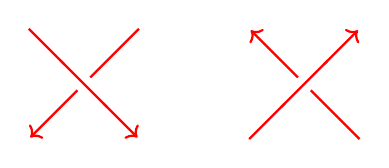
\begin{tikzpicture}[scale=0.7]
					\begin{knot}[clip width=8]
% 						\strand[thick, red] (-3,-0.1) to (-3,2.1);
% 						\strand[thick, red] (-1,-0.1) to (-1,2.1);
						\strand[thick, red, <-] (0,0) to (2,2);
						\strand[thick, red, <-] (2,0) to (0,2);
						\strand[thick, red, ->] (4,0) to (6,2);
						\strand[thick, red, ->] (6,0) to (4,2);
% 						\strand[thick, red] (3,-0.1) to (3,2.1);
% 						\strand[thick, red] (5,-0.1) to (5,2.1);
					\flipcrossings{1}
				\end{knot}
% 					\node[ultra thick, red] at (-2,1) {\(\cdots\)};
% 					\node[ultra thick, red] at (4,1) {\(\cdots\)};

% 					\node[below, label={\(p_1\)}] at (-3,-0.7) {};
% 					\node[below, label={\(p_{i-1}\)}] at (-1,-0.7) {};
% 					\node[below, label={\(q_1\)}] at (-3,2) {};
% 					\node[below, label={\(q_{i-1}\)}] at (-1,2) {};
% 					\node[below, label={\(q_i\)}] at (0,2) {};
% 					\node[below, label={\(q_{i+1}\)}] at (2,2) {};
% 					\node[below, label={\(p_i\)}] at (0,-0.7) {};
% 					\node[below, label={\(p_{i+1}\)}] at (2,-0.7) {};
% 					\node[below, label={\(p_{i+2}\)}] at (3,-0.7) {};
% 					\node[below, label={\(p_{n}\)}] at (5,-0.7) {};
% 					\node[below, label={\(q_{i+2}\)}] at (3,2) {};
% 					\node[below, label={\(q_{n}\)}] at (5,2) {};

% 					\node at (1, -1.1) {\(\sigmaa_i^{-1}\)};
			\end{tikzpicture}}

% 			\caption*{Generators \(\sigmaa_i\) and \(\sigmaa_i^{-1}\)}
			\label{fig:geometricbraidgeneratorssign}
		\end{figure}

		Writhe is the sum of the assigned numbers.
	\end{frame}

% 	\section{Markov trace}

	\begin{frame}
% 		\frametitle{Markov trace}
		Bracket polynomial of a braid:
		\begin{align*}
			\langle \cdot \rangle &\colon \B_n \rightarrow \Z[A, A^{-1}]\\
			\langle \cdot \rangle &\colon b \mapsto \langle \overline{b}\hspace{1pt}\rangle
		\end{align*}
		\(\langle \cdot \rangle\) is well defined and invariant under conjugation.\vspace{20pt}

		Normalisation using writhe:
		\[L(K) \coloneq (-A^3)^{-w(b)}\langle \overline{b}\hspace{1pt}\rangle\]
	\end{frame}

	\begin{frame}
		\[\left\langle\BPB\right\rangle = A\left\langle\BPD\right\rangle + A^{-1}\left\langle\BPE\right\rangle\]\vspace{5pt}

		\[\BPE = \I_n \quad\text{ and }\quad \U_i \coloneq \BPD\]\vspace{10pt}

		\[\left\langle{\sigmaa_{i}^{-1}}\right\rangle = A\braket<\mathrm{U}_i> + A^{-1}\braket<\I_n>\]

		\[\braket<\sigmaa_i> = A\braket<\I_n> + A^{-1}\braket<\mathrm{U}_i>\]
	\end{frame}

	\begin{frame}
		We refer to \(\U_i\)'s as ``hooks'' or ``input-output'' forms.\vspace{10pt}

		They don't belong to the Artin braid group.\vspace{20pt}

		\begin{figure}
			\centering
			\subcaptionbox*{\(U_1\)}{
				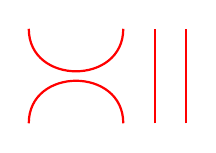
\begin{tikzpicture}[scale=2]
					\draw[thick, red] (-0.3,0.3) .. controls (-0.3,-0.06) and (0.3,-0.06) .. (0.3,0.3);
					\draw[thick, red] (-0.3,-0.3) .. controls (-0.3,0.06) and (0.3,0.06) .. (0.3,-0.3);
					\draw[thick, red] (0.5,-0.3) -- (0.5,0.3);
					\draw[thick, red] (0.7,-0.3) -- (0.7,0.3);
				\end{tikzpicture}}
			\quad\quad\quad\subcaptionbox*{\(U_2\)}{
				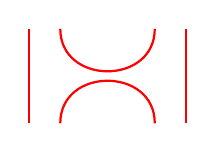
\begin{tikzpicture}[scale=2]
					\begin{knot}[clip width = 5]
						\draw[thick, red] (-0.5,-0.3) -- (-0.5,0.3);
						\draw[thick, red] (-0.3,0.3) .. controls (-0.3,-0.06) and (0.3,-0.06) .. (0.3,0.3);
						\draw[thick, red] (-0.3,-0.3) .. controls (-0.3,0.06) and (0.3,0.06) .. (0.3,-0.3);
						\draw[thick, red] (0.5,-0.3) -- (0.5,0.3);
					\end{knot}
				\end{tikzpicture}}
			\quad\quad\quad\subcaptionbox*{\(U_3\)}{
				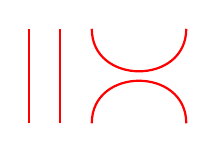
\begin{tikzpicture}[scale=2]
					\begin{knot}[clip width = 5]
						\draw[thick, red] (-0.5,-0.3) -- (-0.5,0.3);
						\draw[thick, red] (-0.3,0.3) .. controls (-0.3,-0.06) and (0.3,-0.06) .. (0.3,0.3);
						\draw[thick, red] (-0.3,-0.3) .. controls (-0.3,0.06) and (0.3,0.06) .. (0.3,-0.3);
						\draw[thick, red] (-0.7,-0.3) -- (-0.7,0.3);
					\end{knot}
				\end{tikzpicture}}
			\caption*{Input-output forms or hooks for 4 strands}
			\label{fig:inputoutputforms}
		\end{figure}
	\end{frame}

	\begin{frame}
		\frametitle{Example}
		\begin{figure}
			\centering
			\subcaptionbox*{\(b\)}{
				\begin{tikzpicture}
					\begin{knot}[clip width=5]
						\strand[very thick, beamer@blendedblue] (2,0) to [out=90,in=-90] (1,1);
						\strand[very thick, beamer@blendedblue] (1,1) [out=90,in=-90] to (0,2);
						\strand[very thick, beamer@blendedblue] (1,0) to [out=90,in=-90] (2,1);
						\strand[very thick, beamer@blendedblue] (2,1) [out=90,in=-90] to (2,2);
						\strand[very thick, beamer@blendedblue] (0,0) to [out=90,in=-90] (0,1);
						\strand[very thick, beamer@blendedblue] (0,1) [out=90,in=-90] to (1,2);
						\flipcrossings{2}
					\end{knot}
				\end{tikzpicture}}
			\quad\quad\quad\subcaptionbox*{\(\overline{b}\)}{
				\begin{tikzpicture}
					\begin{knot}[clip width=5]
						\strand[very thick, beamer@blendedblue] (2,0) to [out=90,in=-90] (1,1);
						\strand[very thick, beamer@blendedblue] (1,1) [out=90,in=-90] to (0,2);
						\strand[very thick, beamer@blendedblue] (1,0) to [out=90,in=-90] (2,1);
						\strand[very thick, beamer@blendedblue] (2,1) [out=90,in=-90] to (2,2);
						\strand[very thick, beamer@blendedblue] (0,0) to [out=90,in=-90] (0,1);
						\strand[very thick, beamer@blendedblue] (0,1) [out=90,in=-90] to (1,2);
						\strand[thick, red] (2,2) to (2,2.5) to (2.5, 2.5) to (2.5,-0.5) to (2,-0.5) to (2,0);
						\strand[thick, red] (1,2) to (1,3) to (3,3) to (3,-1) to (1,-1) to (1,0);
						\strand[thick, red] (0,2) to (0,3.5) to (3.5,3.5) to (3.5,-1.5) to (0,-1.5) to (0,0);
						\flipcrossings{2}
					\end{knot}
				\end{tikzpicture}}
			\label{fig:inputoutputexampleone}
		\end{figure}
	\end{frame}

	\begin{frame}
		\frametitle{Example (contd.)}
		\begin{figure}
		    \centering
			\subcaptionbox*{\(s = \overline{U_1 U_2}\)}{
				\begin{tikzpicture}
					\begin{knot}[clip width=5]
						\draw[very thick, beamer@blendedblue] (1,0) .. controls (1,0.5) and (2,0.5) .. (2,0);
						\draw[very thick, beamer@blendedblue] (1,1) .. controls (1,0.5) and (2,0.5) .. (2,1) to (2,2);
						\draw[very thick, beamer@blendedblue] (0,0) to (0,1) .. controls (0,1.5) and (1,1.5) .. (1,1);
						\draw[very thick, beamer@blendedblue] (0,2) .. controls (0,1.5) and (1,1.5) .. (1,2);
						\strand[thick, red] (2,2) to (2,2.5) to (2.5, 2.5) to (2.5,-0.5) to (2,-0.5) to (2,0);
						\strand[thick, red] (1,2) to (1,3) to (3,3) to (3,-1) to (1,-1) to (1,0);
						\strand[thick, red] (0,2) to (0,3.5) to (3.5,3.5) to (3.5,-1.5) to (0,-1.5) to (0,0);
					\end{knot}
				\end{tikzpicture}}
			\quad\quad\quad\subcaptionbox*{\(U_1 U_2\)}{
				\begin{tikzpicture}
					\begin{knot}[clip width=5]
						\draw[very thick, beamer@blendedblue] (1,0) .. controls (1,0.5) and (2,0.5) .. (2,0);
						\draw[very thick, beamer@blendedblue] (1,1) .. controls (1,0.5) and (2,0.5) .. (2,1) to (2,2);
						\draw[very thick, beamer@blendedblue] (0,0) to (0,1) .. controls (0,1.5) and (1,1.5) .. (1,1);
						\draw[very thick, beamer@blendedblue] (0,2) .. controls (0,1.5) and (1,1.5) .. (1,2);
					\end{knot}
				\end{tikzpicture}}
			\caption*{Writing a state of a braid closure in terms of input-output forms}
			\label{fig:inputoutputexampletwo}
		\end{figure}
	\end{frame}

	\begin{frame}
		\[\braket<b> = \braket<S(b)> = \sum_s \braket<b|s> \braket<P_s> = \sum_s \braket<b|s>\hspace{1pt}\updelta^{\hspace{1pt}\norm{s}}\]\vspace{5pt}

		\[\begin{array}{rll}
			\left\langle S(b) \right\rangle &:& \text{ Substituting } \left\langle \sigmaa_i \right\rangle = A\left\langle \I_n \right\rangle + A^{-1}\left\langle \mathrm{U}_i \right\rangle \text{ and } \vspace{5pt}\\
			& & \left\langle{\sigmaa_{i}^{-1}}\right\rangle = A\left\langle\mathrm{U}_i \right\rangle + A^{-1}\left\langle \I_n \right\rangle \vspace{5pt}\\

			s &:& \text{ A state in the expansion }\vspace{5pt}\\

			P_s &:& \text{ Product of } \U_i \text{'s }\vspace{5pt}\\

			\left\langle b|s \right\rangle &:& \text{ Product of } A\text{'s and } A^{-1}\text{'s}\vspace{5pt}\\

			\updelta &:& \hspace{2pt}-A^2 - A^{-2}\vspace{5pt}\\

			\norm{s} &:& \text{ Number of loops in } s \text{ minus one }
		\end{array}\]
	\end{frame}

	\section{Temperley--Lieb algebra}

	\begin{frame}
		\frametitle{Temperley--Lieb algebra \(\TL_n\)}
		We give \(\U_i\)'s a structure of their own by constructing
		\begin{itemize}
		    \item over the ring \(\Z[A, A^{-1}]\)
			\item the free additive algebra \(\TL_n\)
			\item with the generators \(\U_1, \U_2,\ldots, \U_{n-1}\)
			\item and the multiplicative relations coming from the interpretation of \(\U_i\)'s as input-output forms.
		\end{itemize}\vspace{10pt}
	\end{frame}

	\begin{frame}
		\frametitle{Multiplicative relations in \(\TL_n\)}
		Multiplicative relations in \(\TL_n\):\vspace{10pt}
		\begin{enumerate}
			\item \(\U_i\hspace{1pt}\U_{i\pm 1}\hspace{1pt}\U_i = \U_i\)
			\item \(\U_i^2 = \updelta\hspace{1pt} \U_i\)
			\item \(\U_i\hspace{1pt}\U_j = \U_j\hspace{1pt}\U_i\) if \(\abs{i-j} \geq 2\)
		\end{enumerate}
	\end{frame}

	\begin{frame}
		\frametitle{Geometric interpretation of \(\U_1\U_2\U_1 = \U_1\)}
		\begin{figure}
			\centering
			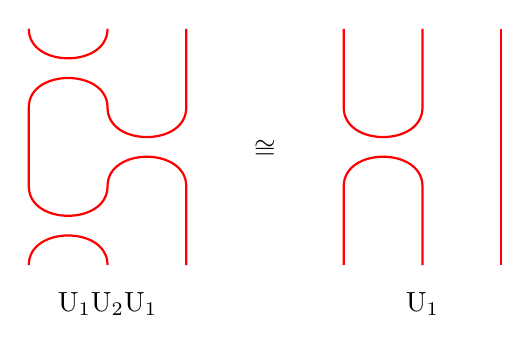
\begin{tikzpicture}
				\begin{knot}[clip width=5]
					\draw[thick, red] (0,0) .. controls (0,0.5) and (1,0.5) .. (1,0);
					\draw[thick, red] (2,0) to (2,1) .. controls (2,1.5) and (1,1.5) .. (1,1) .. controls (1,0.5) and (0,0.5) .. (0,1) to (0,2) .. controls (0,2.5) and (1,2.5) .. (1,2) .. controls (1,1.5) and (2,1.5) .. (2,2) to (2,3);
					\draw[thick, red] (0,3) .. controls (0,2.5) and (1,2.5) .. (1,3);
					\node[label={\(\cong\)}] at (3,1.1) {};
					\draw[thick, red] (4,0) -- (4,1) .. controls (4,1.5) and (5,1.5) .. (5,1) -- (5,0);
					\draw[thick, red] (4,3) -- (4,2) .. controls (4,1.5) and (5,1.5) .. (5,2) -- (5,3);
					\draw[thick, red] (6,0) -- (6,3);
				\end{knot}
				\node at (1,-0.5) {\(\U_1\U_2\U_1\)};
				\node at (5,-0.5) {\(\U_1\)};
			\end{tikzpicture}
			\caption*{Geometric interpretation of \(\U_1\U_2\U_1 = \U_1\)}
			\label{fig:inputoutputillus}
		\end{figure}
	\end{frame}

	\begin{frame}
		\frametitle{Geometric interpretation of \(\U_i^2 = \updelta\hspace{1pt} \U_i\)}
		\begin{figure}
		    \centering
			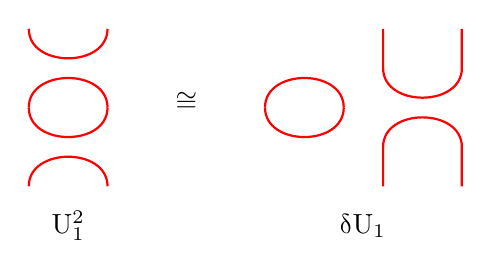
\begin{tikzpicture}
				\draw[thick, red] (0,2) .. controls (0,1.5) and (1,1.5) .. (1,2);
				\draw[thick, red] (0,1) .. controls (0,1.5) and (1,1.5) .. (1,1);
				\draw[thick, red] (0,0) .. controls (0,0.5) and (1,0.5) .. (1,0);
				\draw[thick, red] (0,1) .. controls (0,0.5) and (1,0.5) .. (1,1);
				\node[label={\(\cong\)}] at (2,0.7) {};
				\draw[thick, red] (3,1) .. controls (3,1.5) and (4,1.5) .. (4,1);
				\draw[thick, red] (3,1) .. controls (3,0.5) and (4,0.5) .. (4,1);
				\draw[thick, red] (4.5,0) to (4.5,0.5) .. controls (4.5,1) and (5.5,1) .. (5.5,0.5) -- (5.5,0);
				\draw[thick, red] (4.5,2) to (4.5,1.5) .. controls (4.5,1) and (5.5,1) .. (5.5,1.5) -- (5.5,2);
				\node at (0.5,-0.5) {\(\U_1^2\)};
				\node at (4.25,-0.5) {\(\updelta\hspace{1pt}\U_1\)};
			\end{tikzpicture}
			\caption*{Geometric interpretation of \(\U_i^2 = \updelta\hspace{1pt} \U_i\)}
		\end{figure}
	\end{frame}

	\begin{frame}
		\frametitle{Geometric interpretation of \(\U_3\U_1 = \U_1\U_3\)}
		\begin{figure}
			\centering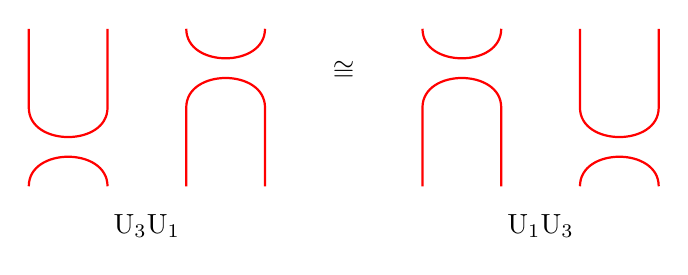
\begin{tikzpicture}
				\draw[thick, red] (0,0) .. controls (0,0.5) and (1,0.5) .. (1,0);
				\draw[thick, red] (0,2) -- (0,1) .. controls (0,0.5) and (1,0.5) .. (1,1) -- (1,2);
				\draw[thick, red] (2,0) -- (2,1) .. controls (2,1.5) and (3,1.5) .. (3,1) -- (3,0);
				\draw[thick, red] (2,2) .. controls (2,1.5) and (3,1.5) .. (3,2);
				\node[label={\(\cong\)}] at (4,1.1) {};
				\draw[rotate around={180:(5.5,1)}, xshift=5cm, thick, red] (0,0) .. controls (0,0.5) and (1,0.5) .. (1,0);
				\draw[rotate around={180:(5.5,1)}, xshift=5cm, thick, red] (0,2) -- (0,1) .. controls (0,0.5) and (1,0.5) .. (1,1) -- (1,2);
				\draw[rotate around={180:(7.5,1)}, xshift=5cm, thick, red] (2,0) -- (2,1) .. controls (2,1.5) and (3,1.5) .. (3,1) -- (3,0);
				\draw[rotate around={180:(7.5,1)}, xshift=5cm, thick, red] (2,2) .. controls (2,1.5) and (3,1.5) .. (3,2);
				\node at (1.5,-0.5) {\(\U_3\U_1\)};
				\node[xshift=5cm] at (1.5,-0.5) {\(\U_1\U_3\)};
			\end{tikzpicture}
			\caption*{Geometric interpretation of \(\U_3\U_1 = \U_1\U_3\)}
		\end{figure}
	\end{frame}

	\begin{frame}
		\frametitle{Representation of \(\B_n\) in \(\TL_n\)}
		We define a mapping \[\uprho \hspace{1pt}\colon \B_n \rightarrow \TL_n\] by
		\begin{align*}
			\uprhoo \hspace{2pt}(\sigmaa_i) &= A + A^{-1}\U_i\\
			\uprhoo \hspace{2pt}(\sigmaa_i^{-1}) &= A^{-1} + A\U_i
		\end{align*}\vspace{10pt}

		\(\uprhoo \hspace{1pt}\colon \B_n \rightarrow \TL_n\) is a representation of the Artin braid group.
	\end{frame}

	\begin{frame}
		\frametitle{Trace}
		We define the diagrammatic trace \[\tr \colon \TL_n \rightarrow \Z[A, A^{-1}]\] by extending linearly \[\tr(P) = \braket<P>.\]\vspace{10pt}

		This version of trace is diagrammatic in nature as we are counting loops in a state.\vspace{10pt}

		\[\braket<b> = \tr(\operatorname{\uprho}\hspace{2pt}(b))\]
	\end{frame}

	\begin{frame}
		\frametitle{Whole procedure}
		So one can\vspace{10pt}
		\begin{itemize}
			\item find a braid representation \(b\) of a link \(L\) by Alexander's theorem,\vspace{10pt}
			\item calculate \(\tr(\operatorname{\uprho}\hspace{2pt}(b))\)\vspace{10pt}
			\item and normalise it to get the link invariant normalised bracket polynomial.\vspace{10pt}
		\end{itemize}\vspace{10pt}

		The substitution \(A = t^{-1/4}\) yields us the Jones polynomial.
	\end{frame}








\end{document}
